\documentclass[12pt]{TD-CJS}
 \renewcommand{\baselinestretch}{2}
 
\usepackage{latexsym}
\usepackage{amsmath}
\usepackage{amsfonts}
\usepackage{amssymb}
\usepackage{psfrag}
\usepackage{graphicx}
\usepackage{enumitem}



\newcommand{\prox}{ \mathop{\mathrm{prox}} }
\newcommand{\R}{\mathcal{R}}
\newcommand{\defeq}{\mathrel{\mathop:}=}
\newcommand{\eqdist}{\stackrel{D}{=}}

\DeclareMathOperator*{\argmax}{arg\,max} 
\DeclareMathOperator*{\argmin}{arg\,min} 

\begin{document}
%\rhauthor{Michael A. Newton,  Nicholas G. Polson and Jianeng Xu}
\rhauthor{BlindedA, BlindedB, and BlindedC}
\copyrightline{Statistical Society of Canada}
\Frenchcopyrightline{Soci\'et\'e statistique du Canada}


\title{Weighted Bayesian Bootstrap for Scalable Bayes}
%\author{Michael Newton\authorref{1}}
%author{Nicholas G. Polson\authorref{2}}
%\author{Jianeng Xu\authorref{3}}
%\affiliation[1]{Departments of Statistics and of Biostatistics and Medical Informatics, University of Wisconsin-Madison}
%\affiliation[2]{Booth School of Business, University of Chicago}
%\affiliation[3]{Booth School of Business, University of Chicago}
\author{BlindedA}
\author{BlindedB}
\author{BlindedC}


\startabstract{
\keywords{
\KWDtitle{Key words and phrases}
Bayesian\sep Bootstrap\sep MCMC\sep Weighted Bootstrap\sep ABC\sep Trend Filtering\sep Deep Learning\sep TensorFlow\sep Regularization.
% MSC 2010 subject classification codes
\KWDtitle{MSC 2010}Primary 62F40\sep secondary 6262F15}
\begin{abstract}
\abstractsection{}
\abstractsection{Abstract}
We develop a weighted Bayesian Bootstrap (WBB) for  machine learning and statistics. WBB provides uncertainty quantification by sampling from a high dimensional posterior distribution. WBB is computationally fast and scalable using only off-the-shelf optimization software such as TensorFlow. We provide regularity conditions which apply to a wide range of machine learning and statistical models. We illustrate our methodology in regularized regression, trend filtering and deep learning. Finally, we conclude with directions for future research.

\end{abstract}}
\makechaptertitle



\newpage

\section{Introduction}
Weighted Bayesian Bootstrap (WBB) is a simulation-based algorithm for assessing uncertainty in machine learning and statistics. Uncertainty quantification (UQ) is an active area of research, particularly in high-dimensional inference 
problems. Whilst there are computationally fast and scalable algorithms for training models in a wide variety of contexts, uncertainty assessments are still required, as are methods to compute these assessments.  Bayesian analysis
offers a general approach, but developing computationally fast scalable algorithms for sampling a posterior distribution is a notoriously hard problem. WBB makes a contribution to this literature by showing how off-the-shelf optimization algorithms, such as convex optimization or stochastic gradient descent (SGD), can be adapted to 
provide uncertainty assessments.
 
Our work builds on \cite{newton1994approximate} who provide a weighted likelihood Bootstrap (WLB) method for Bayesian inference. They develop a sampling algorithm together with asymptotic analysis to show that  the WLB
provides approximate posterior samples. Their bootstrap procedure exploits tools to maximize likelihoods and 
theoretical connections between posterior variation and curvature of log-likelihood revealed through
repeated optimization of randomly weighted likelihoods. 
 By contrast, the proposed weighted Bayesian Bootstrap (WBB) calculates a series of
randomized  posterior modes rather than randomized likelihood maximizers. A key rationale for this proposal is  that 
high dimensional posterior modes are now readily computable, thanks to systems such as TensorFlow and Keras
that deploy stochastic gradiant descent (SGD) and convex optimizaton methods (cites) for large-scale
problems, such as on neural network architectures used in deep learning (cite).
By linking random weighting with modern-day optimization to calibrate estimates, we provide a 
framework for uncertainty quantification.

Quantifying uncertainty is typically unavailable in a purely regularization optimization method. 
From the proposed Bayesian perspective, UQ is 
available directly through repeated optimization of randomized objective functions, using the same
computational tools that produce the primary estimate,  rather than through Markov
chain Monte Carlo, variational methods,  approximate Bayesian computation, or other techniques. 
Thus, uncertainty assessments are provided at little extra computational cost over the original
training computations.  Another useful feature is that  it is straightforward to add a regularization path across hyper-parameters, which is usually difficult to compute in traditional Bayesian
sensitivity analysis.  We use predictive cross-validation techniques in this regard.

The rest of the paper is outlined as follows. Section 2 develops our weighted Bayesian Bootstrap (WBB) algorithm. Section 3 provides applications to high dimensional sparse regression, trend filtering and deep learning. WBB can also be applied to Bayesian tree models (Taddy et al., 2015). Finally, Section 4 concludes with directions for future research. Areas for future study include bootstrap filters in state-space models (Gordon{,}  Salmond \& Smith, 1993)  and comparison with the resampling-sampling
perspective to sequential Bayesian inference (Lopes, Polson \& Carvalho, 2012), etc.

\section{Weighted Bayesian Bootstrap}
Let  $y=(y_1, y_2, \cdots, y_n)$ be an $n$-vector of outcomes and let $\theta$ be a $d$-dimensional parameter of interest. 
Auxiliary data may include a 
fixed $n \times d$ matrix $A$ whose rows are the design points (or ``features'') $a_i^T$
where we index  observations by $i$ and parameters by $j$.  
A large number of machine learning and statistical problems can be expressed in the form
\begin{equation}
\label{eqn:canonicalform}
\begin{aligned}
& \underset{\theta \in \R^d}{\text{minimize}}
& &  l(y| \theta) + \lambda\phi(\theta) \, ,
\end{aligned}
\end{equation}
where $l(y| \theta) = \sum_{i=1}^n l_i( y_i | \theta )$ is a measure of fit (or ``empirical risk function'') depending on $\theta$ and $y$ and implicitly on $A$.
The penalty function or regularization term, $\lambda\phi(\theta) $,  
effects a favorable bias-variance tradeoff.  We allow for the possibility that $\phi(\theta)$ may have points in its domain where it fails to be differentiable.  
If we treat the data, $y$, as arising from a probabilistic 
model parameterized by $\theta$, then the likelihood function $p(y|\theta)$ yields 
the model-associated measure of fit $l(y| \theta) = -\log p(y|\theta)$.
We will make use of the following notation: $ \hat{\theta}_n \defeq {\rm arg max}_\theta\; p(y |\theta) $ to
denote the MLE, and, relative some prior $p(\theta)$,
\begin{enumerate}[label=(\roman*)]
\item let $\theta^*_n \defeq {\rm arg max}_\theta \; p( \theta|y) $ be the posterior mode,
\item let $ \bar{\theta}_n \defeq E(\theta | y) $ be the posterior mean.
\end{enumerate}
Next, we recall a key duality between regularization and Bayesian analysis.

\subsection{Bayesian Regularization Duality}

From the Bayesian perspective, the measure of fit, $l(y|\theta) = - \log p(y| \theta)$, and the penalty function, $\lambda\phi(\theta)$, correspond to the negative logarithms of the likelihood and prior distribution in the model
\begin{align*}
 p(y | \theta) \propto \exp & \{-  l(y|\theta)\} \; , \quad p(\theta) \propto \exp\{ - \lambda\phi(\theta) \} \\
p( \theta | y ) &  \propto \exp\{- ( l(y|\theta) + \lambda\phi(\theta) ) \}.
\end{align*}

The prior is not necessarily proper but the posterior, $p(\theta | y) \propto p(y | \theta) p(\theta)$, may still be proper. This provides an equivalence between regularization and Bayesian methods. For example, regression with a least squares log-likelihood subject to a penalty such as an $L^2$-norm (ridge) Gaussian probability model or $ L^1$-norm (lasso) double exponential probability model. We then have
\begin{eqnarray}
&\hat\theta_n =& \underset{\theta \in \Theta}{\argmin}\, l(y|\theta),\\
&\theta^*_n =& \underset{\theta \in \Theta}{\argmin}\,  \{ l(y|\theta) + \lambda\phi(\theta) \}.  \label{posterior mode}
\end{eqnarray}

Let $\partial$ be the subdifferential operator.  Then a necessary and sufficient condition for $\theta^*$ to minimize $ l(y|\theta) + \lambda\phi(\theta)$  is 
\begin{equation}
\label{eqn:subdiffproxgrad}
0 \in \partial \left\{ l(y|\theta) + \lambda\phi(\theta)\right\} = \nabla l(y|\theta) + \lambda\partial \phi(\theta) 
\end{equation}
the sum of a point and a set.  The optimization literature  characterizes $\theta^*$ as the fixed point of a proximal operator
$\theta^* = \prox_{\gamma \phi}\{ \theta^* - \lambda \nabla f(\theta^*) \} $, see \cite{polson2015mixtures} and \cite*{polson2015proximal} for further discussion. 

A general class of natural exponential family models can be expressed in terms of the Bregman divergence of the dual of the cumulant transform.
Let $ \phi $ be the conjugate Legendre transform of $\psi$. Hence $ \psi(\theta) = \sup_\mu \; \left ( \mu^\top \theta - \phi(\mu) \right )$. Then we can write
\begin{align*}
p_\psi ( y | \theta ) & = \exp \left ( y^\top \theta - \psi( \theta) - h_\psi(y) \right )\\
 & = \exp \left \{ \inf_\mu \; \left ( ( y - \mu )^\top \theta - \phi(\mu) \right ) - h_\psi(y) \right \}\\
& = \exp \left ( - D_\phi ( y , \mu(\theta) ) - h_\phi (y) \right )
\end{align*}
where the infimum is attained at $ \mu(\theta) = \phi^\prime (\theta) $ is the mean of the exponential family distribution. 
We rewrite $ h_\psi(y) $ is terms of the correction term and $ h_\phi(y)$. Here there is a duality as $D_\phi$ can be interpreted as a Bregman divergence. 

For a wide range of non-smooth objective functions/statistical models, recent regularization methods provide fast, scalable algorithms for calculating estimates of the form (\ref{posterior mode}), which can also be viewed as the posterior mode. Therefore as $\lambda$ varies we obtain a full regularization path as a form of prior sensitivity analysis. 

\cite{strawderman2013hierarchical} and  \cite{polson2015proximal} considered scenarios where posterior modes can be used as posterior means from augmented probability models. Moreover, in their original foundation of the Weighted Likelihood Bootstrap (WLB), \cite{newton1994approximate} introduced the concept of the implicit prior. Clearly this is an avenue for future research. 

\subsection{WBB Algorithm}
\noindent We now define the weighted Bayesian Bootstrap (WBB). Following \cite{newton1994approximate}, we construct a randomly weighted posterior distribution denoted by
$$
{\bf w} = (w_1, ..., w_n, w_p),\,
p_{\bf w}(\theta | y) \propto \prod_{i=1}^n p(y_i|\theta)^{w_i} p(\theta)^{w_p}
$$
where the weights $w_p, w_i \sim Exp(1)$ are randomly generated weights. It's equivalent to draw
$w_i = \log(1/U_i)$ where $U_i$'s are i.i.d. Uniform (0,1), which is motivated by the uniform Dirichlet distribution for multinomial data. We have used the fact that for i.i.d. observations, the likelihood can be factorized as $p(y|\theta) = \prod_{i=1}^n p(y_i|\theta)$. This is not crucial for our analysis but is a common assumption. Let $\theta^*_{{\bf w},n}$ denote the mode of this regularized distribution. Again, there is an equivalence 
$$
\theta^*_{{\bf w},n} := \underset{\theta}{\argmax} \; p_{\bf w}(\theta | y) \equiv \underset{\theta}{\argmin} \sum_{i=1}^n w_i l_i(y_i|\theta) + \lambda w_{p} \phi(\theta)
$$
where $l_i(y_i|\theta) = -\log p(y_i|\theta)$ and $ \lambda\phi(\theta) = -\log p(\theta)$. Note that we have a weighted likelihood and a new regularization parameter, $\lambda w_p$.

\noindent  The crux of our procedure is to create a sample of the weighted posterior modes $\{ \theta_{{\bf w},n}^*\}$ (computationally cheap as each sub-problem can be solved via optimization). Our main result is the following:\\
\textbf{Algorithm: Weighted Bayesian Bootstrap (WBB)}
\begin{enumerate}
\item Iterate: sample ${\bf{w}} = \{w_1, w_2, ..., w_n, w_p\}$ via exponentials. $w_p, w_i\sim Exp(1)$. 
\item For each ${\bf{w}}$, solve $\theta^*_{{\bf w},n} = \underset{\theta}{\argmin} \sum_{i=1}^n w_i l_i(\theta) +  \lambda w_p \phi(\theta)$. 
\end{enumerate}

The WBB algorithm is fast and scalable to compute a regularized estimator. For a large number of popular priors, the minimizing solution $\theta^*_{{\bf w},n}$ in the second step can be directly obtained via regularization packages such as {\tt glmnet} by Trevor Hastie and {\tt genlasso} by Taylor Arnold. When the likelihood function or the prior is specially designed, Stochastic Gradient Descent (SGD) is powerful and fast enough to solve the minimization problem. It can be easily implemented in TensorFlow once the objective function is specified. See Appendix and \cite{polson2017deep} for further discussion. 

The next section builds on \cite{newton1994approximate} and derives asymptotic properties of the weighted Bayesian Bootstrap. We simply add the regularized factor. To choose the amount of regularization $\lambda$, we can use the marginal likelihood $m_\lambda (y)$, estimated by bridge sampling (Gelman \& Meng, 1998) or simply using predictive cross-validation.

\subsection{WBB Properties}
The following proposition which follows from the Theorem 2 in \cite{newton1994approximate} summaries the properties of WBB.
\begin{proposition}{Proposition}{}
The weighted Bayesian Bootstrap draws are approximate posterior samples
$$
\left\{\theta^{*(k)}_{{\bf w},n} \right\}_{k=1}^K \sim p(\theta | y).
$$
\end{proposition}

Now we consider `large $n$' properties. The variation in the posterior density $p(\theta|y) \propto e^{-n l_n(\theta)}p(\theta)$ for sufficiently large $n$ will be dominated by the likelihood term. Expanding $l_n(\theta)$ around its maximum, $\hat\theta$, and defining $J_n(\hat\theta) = nj(\hat\theta)$ as the observed information matrix gives the traditional normal approximation for the posterior distribution
$$
\theta \sim N_d \left( \hat\theta_n, J_n^{-1}(\hat\theta)\right)
$$
where $ \hat{\theta}_n$ is the MLE. A more accurate approximation is obtained by expanding around the posterior mode, $\theta^*$, which we will exploit in our weighted Bayesian Bootstrap. Now we have the asymptotic distributional approximation 
$$
\theta \sim N_d \left( \theta^*, J_n^{-1}(\theta^*)\right)
$$
where $\theta^*_n \defeq {\rm arg \; max}_\theta \; p( \theta|y) $ is the posterior mode. 

The use of the posterior mode here is crucially important as it's the mode that is computationally available from TensorFlow and Keras (\cite{tensorflow2015-whitepaper,chollet2015keras}). Approximate normality and second order approximation also holds, see \cite{johnson1970asymptotic}, \cite{Bertail} and \cite{newton1994approximate} for future discussion. Specifically,
$$
\sqrt{ n I ( \hat{\theta}_n )} \left ( {\theta}^*_n - \hat{\theta}_n \right ) \eqdist Z
$$
where $Z \sim N(0,1)$ is a standard Normal variable. The conditional posterior satisfies $\mathbb{P} \left ( | {\theta}^*_n - \hat{\theta}_n | > \epsilon \right ) \rightarrow 0$ for each $ \epsilon > 0 $ as $ n \rightarrow \infty $. In the 'large $p$' case, a number of results are available for posterior concentration, for example, see \cite{van2014horseshoe} for sparse high dimensional models.

\section{Applications}
Consider now a number of scenarios to assess when WBB corresponds to a full Bayesian posterior distribution. 
\subsection{Lasso}
First, a simple univariate normal means problem with a  lasso prior where  
$$
y|\theta \sim N(\theta,1^2), \quad \theta \sim Laplace (0,1/\lambda)
$$

Given the i.i.d. exponential weights $w_1$ and $w_2$, the weighted posterior mode $\theta^*_{\bf w}$ is 
$$
\theta^*_{\bf w} = \underset{\theta \in \Theta}{\argmin}\, \left\{\frac{w_1}{2} (y-\theta)^2 + \lambda w_2 |\theta|\right\}.
$$
This is sufficiently simple for an exact WBB solution in terms of soft thresholding:
$$
\theta^*_{\bf w} = 
\begin{cases}
y - \lambda w_2/w_1 &\mbox{if $y > \lambda w_2/w_1$},\\
y + \lambda w_2/w_1 &\mbox{if $y < -\lambda w_2/w_1$},\\
0 &\mbox{if $|y| \leq \lambda w_2/w_1$}.\\
\end{cases}
$$
The WBB mean $E_{{\bf w}}(\theta^*_{\bf w}|y)$ is approximated by the sample mean of $\{ \theta^{*(k)}_{\bf w}\}_{k=1}^K$. On the other hand, \cite{mitchell1994note} gives the expression for the posterior mean, 

\begin{eqnarray*}
E(\theta|y) &=& \frac{\int_{-\infty}^\infty \theta\exp\left\{-(y-\theta)^2/2 - \lambda |\theta|\right\} d\theta}{\int_{-\infty}^\infty \exp\left\{-(y-\theta)^2/2 - \lambda |\theta|\right\} d\theta}\\
&=& \frac{F(y)}{F(y) + F(-y)}(y+\lambda) + \frac{F(-y)}{F(y) + F(-y)}(y-\lambda)\\
&=& y + \frac{F(y) - F(-y)}{F(y) + F(-y)}\lambda
\end{eqnarray*}
where $F(y) = \exp(y)\Phi(-y-\lambda)$ and $\Phi(\cdot)$ is the c.d.f. of standard normal distribution. We plot  the WBB mean versus the exact posterior mean in Figure (\ref{simple}).  Interestingly, WBB algorithm gives sparser posterior means. 

\begin{figure}[!ht]
\centering 
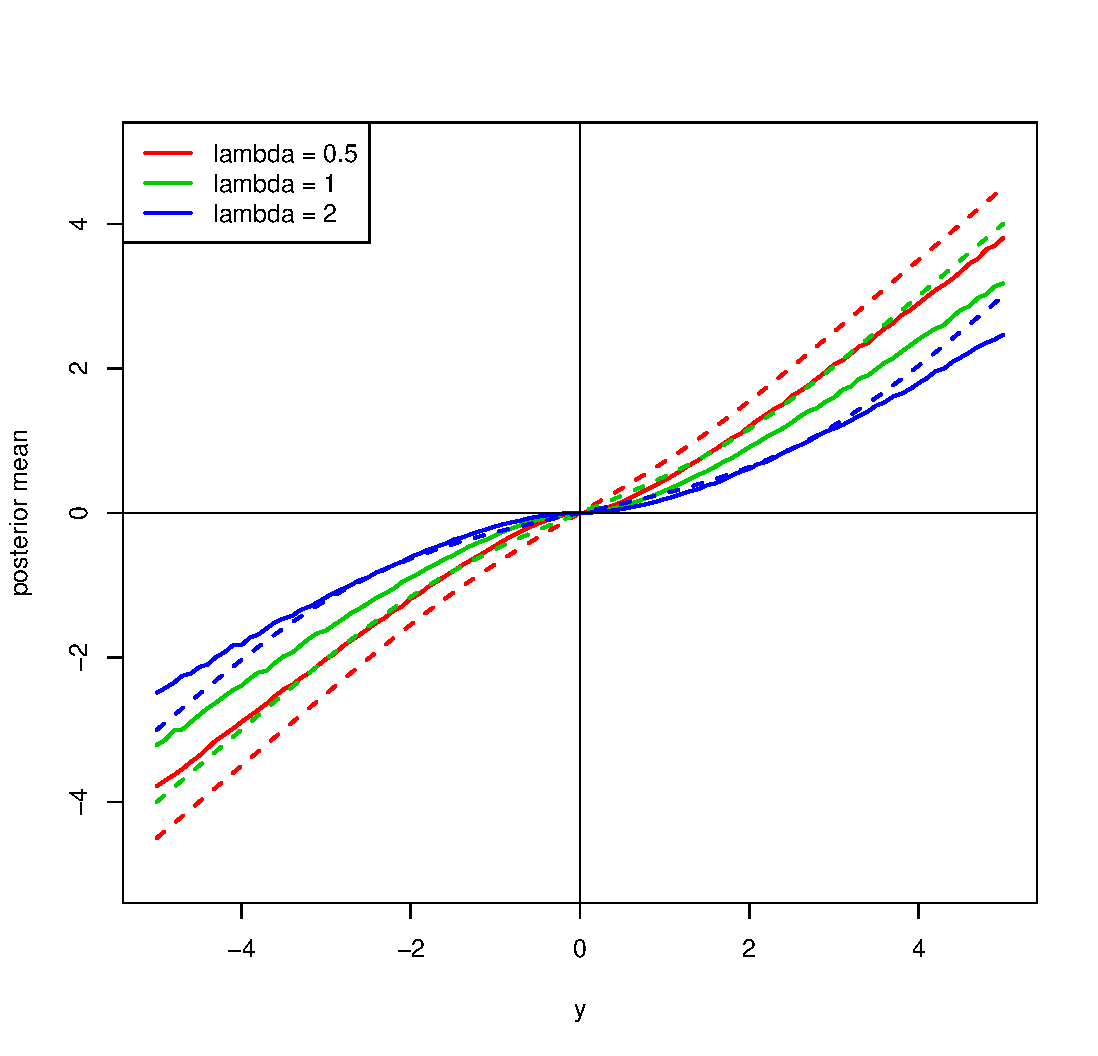
\includegraphics[scale=0.55]{simple.pdf} 
\caption{Normal means model with lasso prior: WBB mean $E_{{\bf w}}(\theta^*_{\bf w}|y)$ (in solid lines) versus exact posterior mean $E(\theta|y)$ (in dashed lines).}
\label{simple}
\end{figure}


\subsection{Diabetes Data}
To illustrate our methodology, we use weighted Bayesian Bootstrap (WBB) on the classic diabetes dataset. The measurements for 442 diabetes patients are obtained ($n=442$), with 10 baseline variables ($p=10$), such as age, sex, body mass index, average blood pressure, and six blood serum measurements. 

The likelihood function is given by
$$
l(y|\beta) = \prod_{i=1}^n p(y_i|\beta)
$$
where
$$
p(y_i|\beta) = \frac{1}{\sqrt{2\pi}\sigma} \exp\left\{-\frac{1}{2\sigma^2}(y_i - x_i'\beta)^2 \right\}.
$$

\noindent We draw 1000 sets of weights ${\bf{w}} = \{w_i\}_{i=1}^{n+1}$ where $w_i$'s are i.i.d. exponentials. For each weight set, the weighted Bayesian estimate $\beta^*_{\bf w}$ is calculated using Equation (\ref{eqn:diabetes}) via the regularization method in the package {\tt glmnet}. 

\begin{equation}
\label{eqn:diabetes}
\hat\beta_{\bf{w}} := \underset{\beta}{\argmin} \;\sum_{i=1}^n w_i(y_i - x_i'\beta)^2+ \lambda w_{n+1}\sum_{j=1}^p |\beta_j|\; . 
\end{equation}
The regularization factor $\lambda$ is chosen by cross-validation with unweighted likelihood. The weighted Bayesian Bootstrap is also performed with fixed prior, namely, $w_{n+1}$ is set to be 1 for all bootstrap samples. \cite{polson2014Bayesian} analyze the same dataset using the Bayesian Bridge estimator and suggest MCMC sampling from the posterior. 

To compare our WBB results we also run the Bayesian bridge estimation. Here the Bayesian setting we use is 
$$p(\beta, \sigma^2) = p(\beta | \sigma^2)p(\sigma^2),\, \text{where }  p(\sigma^2) \propto 1/\sigma^2.$$
The prior on $\beta$, with suitable normalization constant $C_\alpha$, is given by $$p(\beta) = C_\alpha\exp(-\sum_{j=1}^p |\beta_j/\tau|^\alpha  ).$$ The hyper-parameter is drawn as $\nu = \tau^{-\alpha} \sim \Gamma(2,2)$, where $\alpha = 1/2.$\\


\begin{figure}[!ht]
\centering 
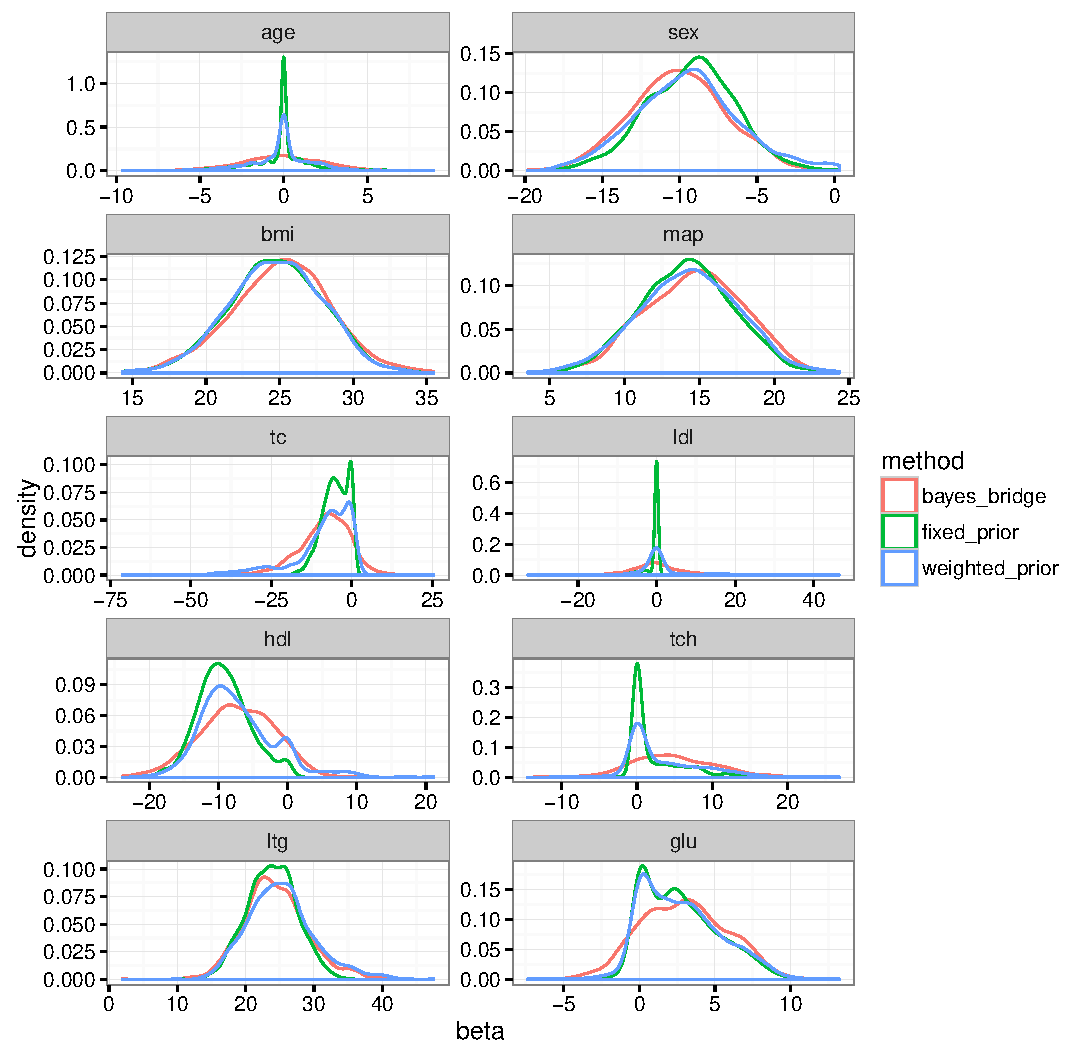
\includegraphics[scale=0.7]{diabetes.pdf} 
\caption{Diabetes example: the weighted Bayesian Bootstrap (with fixed prior and weighted prior) and Bayesian Bridge are used to draw from the marginal posteriors for $\beta_j$'s, j = 1,2,...10. }
\label{diabetes}
\end{figure}

Figure (\ref{diabetes}) shows the results of all these three methods (the weighted Bayesian Bootstrap with fixed prior / weighted prior and the Bayesian Bridge). Marginal posteriors for $\beta_j$'s are presented. One notable feature is that the weighted Bayesian Bootstrap tends to introduce more sparsity than Bayesian Bridge does. For example, the weighted Bayesian Bootstrap posteriors of {\tt age, ldl} and {\tt tch} have higher spikes located around 0, compared with the Bayesian Bridge ones. For {\tt tc, hdl, tch} and {\tt glu}, multi-modes in the marginal posteriors are observed. In general, the posteriors with fixed priors are more concentrated than those with randomly weighted priors. This difference is naturally attributed to variation in the weight assigned to the log-prior penalty term.


\subsection{Trend Filtering}
The generalized lasso solves the optimization problem:
\begin{eqnarray}
\beta^* &=& \underset{\beta}{\argmin} \, \left\{ l(y|\beta) + \lambda\phi(\beta)  \right\}\\
&=& \underset{\beta}{\argmin} \, \frac{1}{2}\|y - X\beta\|_2^2 + \lambda \|D\beta\|_1
\end{eqnarray}
where $ l(y|\beta) = \frac{1}{2}\|y - X\beta\|_2^2 $ is the negative log-likelihood. $D \in \R^{m\times p}$ is a penalty matrix and $ \lambda\phi(\beta) = \lambda \|D\beta\|_1$ is the negative log-prior or regularization penalty. There are fast path algorithms for solving this problem (see {\tt genlasso} package).

As a subproblem, polynomial trend filtering (Tibshirani, 2014; Polson \& Scott, 2015a) is recently introduced for piece-wise polynomial curve-fitting, where the knots and the parameters are chosen adaptively. Intuitively, the trend-filtering estimator is similar to an adaptive spline model: it penalizes the discrete derivative of order $k$, resulting in piecewise polynomials of higher degree for larger $k$.

Specifically, $X = I_p$ in the trend filtering setting  and the data $y = (y_1, ..., y_p)$ are assumed to be meaningfully ordered from 1 to $p$. The penalty matrix is specially designed by the discrete $(k+1)$-th order  derivative,
$$D^{(1)}=
\begin{bmatrix}
    -1       & 1 & 0 & \dots & 0 & 0 \\
    0       & -1 & 1 & \dots & 0 & 0 \\
    \hdotsfor{5} \\
    0       & 0 & 0 & \dots & -1 & 1
\end{bmatrix}_{(p-1)\times p}
$$
and $D^{(k+1)} = D^{(1)}D^{(k)}$ for $k =1,2,3...$. For example, the log-prior in linear trend filtering is explicitly written as $\lambda\sum_{i=1}^{p-2}|\beta_{i+2} - 2\beta_{i+1} + \beta_{i}|$. For a general order $k >1$, 
$$
\|D^{(k+1)}\beta\|_1 = \sum_{i=1}^{p-k-1} \Big| \sum_{j=i}^{i+k+1} (-1)^{(j-i)} \binom{k+1}{j-i}\beta_j \Big|.
$$
WBB solves the following generalized lasso problem in each draw:
\begin{eqnarray*}
 \beta_{\bf w}^* &=& \underset{\beta}{\argmin} \, \frac{1}{2}\sum_{i=1}^p w_i(y_i - \beta_i)^2 + \lambda w_{p+1}\|D^{(k)}\beta\|_1\\
&=&\underset{\beta}{\argmin} \, \frac{1}{2}  \|Wy - W\beta\|_2^2  + \lambda \|D^{(k)}\beta\|_1\\
&=&W^{-1}  \underset{\tilde\beta}{\argmin} \, \frac{1}{2}  \|\tilde{y}_{\bf w} - \tilde{\beta}_{\bf w}\|_2^2  + \lambda \|\tilde{D}^{(k)}_{\bf w}\tilde{\beta}_{\bf w}\|_1\\
\end{eqnarray*}
where $$W = diag(\sqrt{w_i}/\sqrt{w_{p+1}}, ...,  \sqrt{w_p}/\sqrt{w_{p+1}})$$ and $$\tilde{y}_{\bf w} = Wy, \, \tilde{\beta}_{\bf w} = W\beta, \,   \tilde{D}^{(k)}_{\bf w}= D^{(k)}W^{-1}.$$
To illustrate our method, we simulate data $y_i$ from a Fourier series regression 
$$
y_i = \sin\left(\frac{4\pi}{500} i\right)\exp\left({\frac{3}{500} i}\right) + \epsilon_i
$$
for $i=1,2,...500$, where $\epsilon_i\sim N(0,2^2)$ are i.i.d. Gaussian deviates. The cubic trend filtering result is given in Figure (\ref{filter}). 

For each $i$, the WBB gives a group of estimates $\left\{\beta_{\bf w}^*(i) \right\}_{j=1}^T$ where $T$ is the total number of draws. The standard deviation of these weighted solutions consitutes a posterior standard deviation, or
essentially  a standard error for the estimator $\hat \beta_i$.
\begin{figure}[!ht]
\centering 
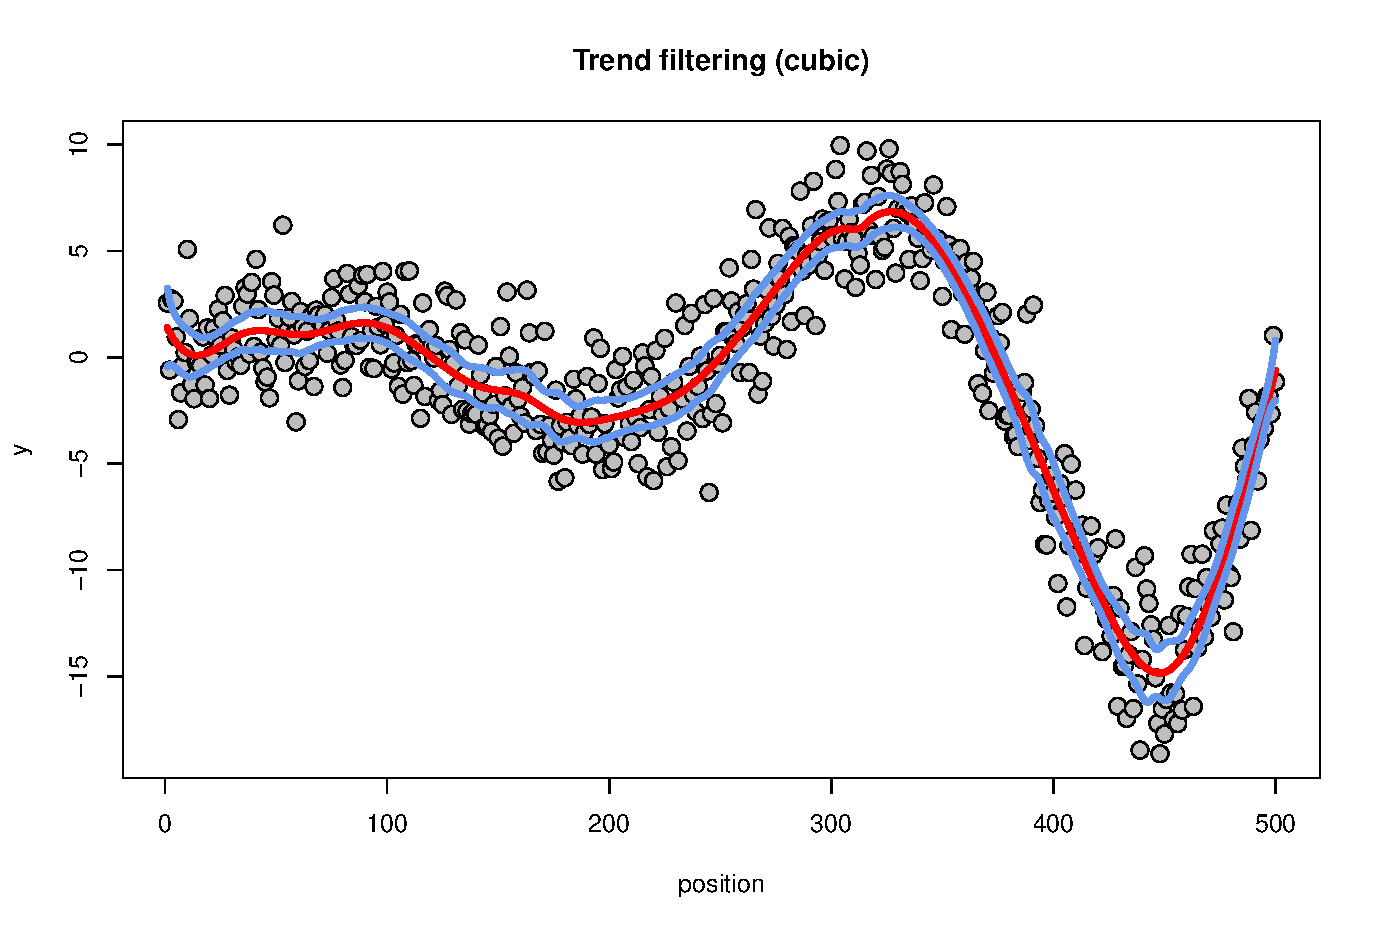
\includegraphics[scale=0.55]{filtering.pdf} 
\caption{Cubic trend filtering: the red line is $\hat\beta_i$ for $i=1,2,...500$; the blue line is $\hat\beta_i \pm 2*se$ where the standard errors are computed by WBB. $\lambda = 1000$.}
\label{filter}
\end{figure}


\subsection{Deep Learning: MNIST Example}
Deep learning is a form of machine learning that uses hierarchical abstract layers of latent variables to perform pattern matching and prediction. \cite{polson2017deep} take a Bayesian probabilistic perspective and provide a number of insights into more efficient algorithms for optimization
and hyper-parameter tuning.

The general goal is to finds a predictor of an output $y$ given a high dimensional input $x$. For a classification problem, $y \in \{1, 2, ..., K\}$ is a discrete variable and can be coded as a $K$-dimensional 0-1 vector. The model is as follows. Let $z^{(l)}$ denote the $l$-th layer, and so $x = z^{(0)}$. The final output is the response $y$,
which can be numeric or categorical. A deep prediction rule is then 
\begin{align*}
z^{(1)} & = f^{(1)} \Big( W^{(0)} x + b^{(0)} \Big),\\
z^{(2)} & = f^{(2)} \Big( W^{(1)} z^{(1)} + b^{(1)} \Big),\\
& \cdots \\
z^{(L)} & = f^{(L)} \Big( W^{(L-1)} z^{(L-1)} + b^{(L-1)} \Big),\\
\hat{y} (x) & = z^{(L)}.
\end{align*}
Here, $W^{(l)}$ are weight matrices, and $b^{(l)}$ are threshold or activation levels. $f^{(l)}$ is the activation function. Probabilistically, the output $y$ in a classification problem is generated by a probability model 
$$
p(y|x, W, b) \propto \exp\{-l(y|x, W, b)\}
$$
where $l(y|x, W, b) = \sum_{i=1}^{n}l_i(y_i|x_i, W, b) $ is the  negative cross-entropy,
$$
l_i(y_i|x_i, W, b) = l_i(y_i, \hat{y}(x_i)) = \sum_{k=1}^K y_{ik}\log\hat{y}_k(x_i)
$$
where $y_{ik}$ is 0 or 1 and $K = 10$.
Adding the negative log-prior $\lambda\phi(W, b)$, the objective function (negative log-posterior) to be minimized by stochastic gradient descent is 
$$
\mathcal{L}_\lambda(y,\hat{y}) = \sum_{i=1}^{n}l_i(y_i, \hat{y}(x_i)) + \lambda\phi(W, b).
$$
Accordingly, with each draw of weights ${\bf w}$, WBB provides the estimates $(W^*_{\bf w}, b^*_{\bf w})$ by solving the following optimization problem.
$$
(W^*_{\bf w}, b^*_{\bf w}) = \argmin_{W, b} \sum_{i=1}^{n}w_i l_i(y_i|x_i, W, b) + \lambda w_p\phi(W, b)
$$

We take the classic MNIST example to illustrate the application of WBB in deep learning. The MNIST database of handwritten digits, available from Yann LeCun's website, has 60,000 training examples and 10,000 test examples. Here the high-dimensional $x$ is a normalized and centered fixed-size ($28\times 28$) image and the output $\hat{y}$ is a 10-dimensional vector, where $i$-th coordinate corresponds to the probability of that image being the $i$-th digit.

For simplicity, we build a 2-layer neural network with layer sizes 128 and 64 respectively. Therefore, the dimensions of parameters are
\begin{align*}
W^{(0)} \in \R^{128\times 784},\, b^{(0)}\in \R^{128},\\
W^{(1)} \in \R^{64\times 128},\, b^{(1)}\in \R^{64},\\
W^{(2)} \in \R^{10\times 64},\, b^{(0)}\in \R^{10}.
\end{align*}
The activation function $f^{(i)}$ is ReLU, $f(x) = \max\{0,x\}$, and the negative log-prior is specified as 
$$
\lambda\phi(W,b) = \lambda\sum_{l=0}^{2}\Vert W^{(l)} \Vert_2^2
$$
where $\lambda = 10^{-4}$. 

Figure (\ref{fig:acc}) shows the posterior distribution of the classification accuracy in the test dataset. We see that the test accuracies are centered around 0.75 and the posterior distribution is left-skewed. Furthermore, the accuracy is higher than 0.35 in 99\% of the cases. The 95\% interval is [0.407, 0.893].

\begin{figure}[!ht]
	\centering
	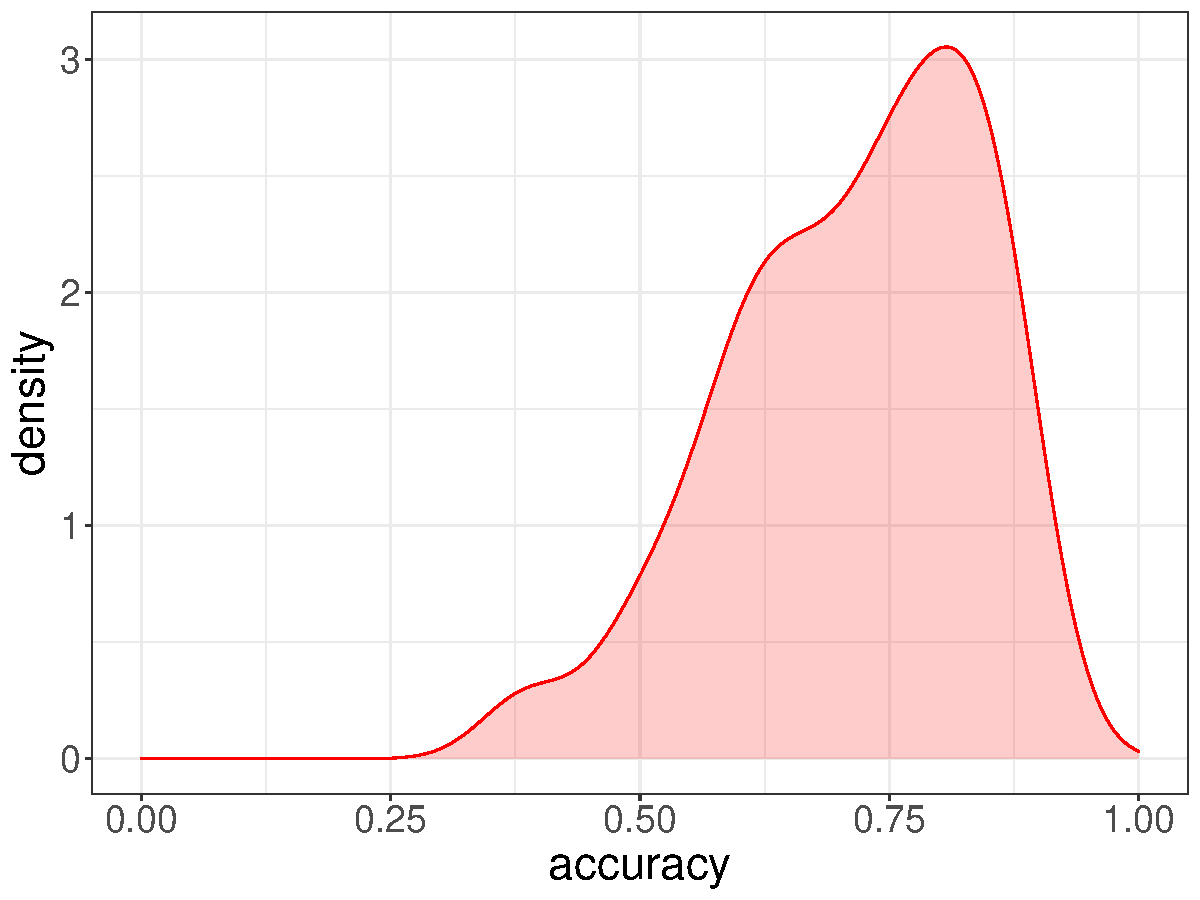
\includegraphics[width=0.7\linewidth]{acc}
	\caption{Posterior distribution of the classification accuracy. $n=500, \lambda=10^{-4}$.}
	\label{fig:acc}
\end{figure}



\section{Discussion}
Weighted Bayesian Bootstrap (WBB) provides a computationally attractive solution to scalable Bayesian inference (Minsker et al., 2014; Welling \& Teh, 2011)
whilst accounting for parameter uncertainty by drawing  samples from a weighted posterior distribution. WBB can also be used in conjunction with proximal methods (Parikh \& Boyd, 2013; Polson \& Scott, 2015b)
to provide  sparsity in high dimensional statistical problems. With a similar ease of computation, WBB provides an alternative to ABC methods (Beaumont, 2009) and Variational Bayes (VB) methods. A fruitful area for future research is the comparison of approximate Bayesian computation with simulated Bayesian Bootstrap inference.

\begin{thebibliography}{}

\bibitem[Beaumont et al., 2009]{beaumont2009adaptive}
Beaumont, M. A.,  Cornuet, J.M.,  Marin,J.M. \& Robert, C. P. (2009). Adaptive approximate bayesian computation. {\it Biometrika}, 96(4), 983--990.

\bibitem[Bertail \& Lo, 1991]{Bertail}
Bertail, P. \& Lo,  A. Y.  (1991). On Johnson's asymptotic expansion for a posterior distribution. {\it Centre de Recherche en Economie et Statistique}.

\bibitem[Daniels \& Young, 1991]{daniels1991saddlepoint}
Daniels, H. \& Young, G.  (1991). Saddlepoint approximation for the studentized mean, with an application to the bootstrap. {\it Biometrika},78(1), 169--179.

\bibitem[Efron, 1981]{efron1981nonparametric}
Efron, B. (1981). Nonparametric standard errors and confidence intervals. {\it Canadian Journal of Statistics}, 9(2), 139--158.

\bibitem[Efron, 2012]{efron2012bayesian}
Efron, B. (2012). Bayesian inference and the parametric bootstrap. {\it The Annals of Applied Statistics}, 6(4), 1971.

\bibitem[Gelman \& Meng, 1998]{gelman1998simulating}
Gelman, A. \& Meng, X.L. (1998). Simulating normalizing constants: From importance sampling to bridge sampling to path sampling. {\it Statistical Science}, 163--185.

\bibitem[Gordon{,}  Salmond \& Smith, 1993]{gordon1993novel}
Gordon, N. J.,  Salmond, D. J. \&  Smith, A. F. (1993). Novel approach to nonlinear/non- gaussian Bayesian state estimation. {\it In IEE Proceedings F (Radar and Signal Processing)}, 140(2) 107--113, IET Digital Library.

\bibitem[Gramacy \& Polson, 2012]{gramacy2012simulation}
Gramacy, R. B. \& Polson, N. G. (2012). Simulation-based regularized logistic regression. {\it Bayesian Analysis }, 7(3), 567--590.

\bibitem[Hans, 2009]{hans2009Bayesian}
Hans, C. (2009). Bayesian lasso regression. {\it Biometrika}, 96(4), 835--845.

\bibitem[Johnson, 1970]{johnson1970asymptotic}
Johnson, R. A. (1970). Asymptotic expansions associated with posterior distributions.
{\it The Annals of Mathematical Statistics}, 41(3), 851--864.

\bibitem[Lopes{,}  Polson \& Carvalho, 2012]{lopes2012bayesian}
Lopes, H. F., Polson, N. G., \&  Carvalho, C. M. (2012). Bayesian statistics with a smile: a resampling-sampling perspective. {\it Brazilian Journal of Probability and Statistics}, 26(4) 358--371.

\bibitem[Minsker et al., 2014]{minsker2014scalable}
Minsker, S., Srivastava, S.,  Lin, L. \& Dunson, D. (2014). Scalable and robust bayesian inference via the median posterior. {\it International Conference on Machine Learning}, 1656--1664.

\bibitem[Mitchell, 1994]{mitchell1994note}
Mitchell, A. F. (1994). A note on posterior moments for a normal mean with double- exponential prior. {\it Journal of the Royal Statistical Society. Series B (Methodological)}, 605--610.

\bibitem[Newton, 1991]{newton1991weighted}
Newton, M. A. (1991). The weighted likelihood bootstrap and an algorithm for prepivoting. Ph. D. thesis, Department of Statistics, University of Washington, Seattle.

\bibitem[Newton \& Raftery, 1994]{newton1994approximate}
Newton, M. A. \& Raftery,, 1994 A. E.  (1994). Approximate Bayesian inference with the weighted likelihood bootstrap. {\it Journal of the Royal Statistical Society. Series B (Methodological)}, 3--48.

\bibitem[Parikh \& Boyd, 2014]{parikh2013proximal}
Parikh, N. \&  Boyd, S. (2014). Proximal algorithms. {\it Foundations and Trends in Optimization}, 1(3), 127--239.

\bibitem[Polson \& Scott, 2015a]{polson2015mixtures}
Polson, N. G. \&  Scott , J. G.(2015). Mixtures, envelopes and hierarchical duality. {\it Journal of the Royal Statistical Society: Series B (Statistical Methodology)},  78(4), 701--727.

\bibitem[Polson \& Scott, 2015b]{polson2015proximal}
Polson, N. G.,  Scott, J. G., \& Willard, B. T.  (2015). Proximal algorithms in statistics and machine learning. {\it Statistical Science}, 30(4), 559--581.

\bibitem[Polson{,}  Scott \& Windle, 2014]{polson2014Bayesian}
Polson, N. G.,  Scott, J. G., \& Windle, J. (2014). The Bayesian bridge. {\it Journal of the Royal Statistical Society: Series B (Statistical Methodology)}, 76(4), 713--733.

\bibitem[Polson \& Sokolov, 2017]{polson2017deep}
Polson, N. G. \&  Sokolov, V. (2017). Deep learning: A bayesian perspective. {\it Bayesian Analysis},12(4), 1275--1304.

\bibitem[Rubin, 1981]{rubin1981Bayesian}
Rubin, D. B. (1981). The Bayesian bootstrap. {\it The Annals of Statistics}, 9(1), 130--134.

\bibitem[Strawderman{,}  Wells \&  Schifano, 2013]{strawderman2013hierarchical}
Strawderman, R. L., Wells, M. T., \& Schifano, E. D. (2013). Hierarchical Bayes, maxi- mum a posteriori estimators, and minimax concave penalized likelihood estimation. {\it Electronic Journal of Statistics}, 7, 973--990.

\bibitem[Taddy et al., 2015]{taddy2015bayesian}
Taddy, M.,  Chen, C.S., Yu, J.  \&  Wyle M. (2015). Bayesian and empirical Bayesian forests. {\it arXiv preprint arXiv:1502.02312}.

\bibitem[Tibshirani, 2014]{tibshirani2014adaptive}
Tibshirani, R. J. (2014). Adaptive piecewise polynomial estimation via trend filtering. {\it The Annals of Statistics}, 42(1), 285--323.

\bibitem[Van Der Pas{,}  Kleijn \& Van Der Vaart, 2014]{van2014horseshoe}
Van Der Pas, S., Kleijn, B.  \&  Van Der Vaart, A. (2014). The horseshoe estimator: Posterior concentration around nearly black vectors. {\it Electronic Journal of Statistics}, 8(2), 2585--2618.

\bibitem[Welling \& Teh, 2011]{welling2011bayesian}
Welling, M. \&  Teh, Y. W. (2011). Bayesian learning via stochastic gradient Langevin dynamics. {\it In Proceedings of the 28th International Conference on Machine Learning} (ICML- 11), 681--688.

\bibitem[West, 1991]{west1992modelling}
West, M. (1991). {\it Modelling with mixtures} Institute of Statistics and Decision Sciences, Duke University
\end{thebibliography}


\begin{appendix}\label{SGD}
Stochastic gradient descent (SGD) method or its variation  is typically used to find the deep learning model weights by minimizing the penalized loss function, $\sum_{i=1}^n w_i l_i(y_i; \theta) + \lambda w_{p} \phi(\theta)$. The method minimizes the function by taking a negative step along an estimate $g^k$ of the gradient $\nabla\left[\sum_{i=1}^n w_i l_i(y_i; \theta^k) + \lambda w_{p} \phi(\theta^k)\right] $ at iteration $k$. 
The approximate gradient is estimated by calculating 
\[
g^k = \frac{n}{b_k} \sum_{i \in E_k} w_i\nabla  l_i(y_i; \theta^k) +  \lambda w_{p} \frac{n}{b_k}\nabla \phi(\theta^k)
\]
Where $E_k \subset \{1,\ldots,n \}$ and $b_k = |E_k|$ is the number of elements in $E_k$. When $b_k >1$ the algorithm is called batch SGD and simply SGD otherwise. A usual strategy to choose subset $E$ is to go cyclically and pick consecutive elements of $\{1,\ldots,T \}$, $E_{k+1} = [E_k \mod n]+1$. The approximated direction  $g^k$ is calculated using a chain rule (aka back-propagation) for deep learning. It  is an unbiased estimator. Thus, at each iteration, the SGD updates the solution
\[
\theta^{k+1} = \theta^k - t_k g^k
\]
For deep learning applications the step size $t_k$ (a.k.a learning rate) is usually kept constant or some simple step size reduction strategy is used, $t_k = a\exp(-kt)$. Appropriate learning rates or the hyperparameters of reduction schedule  are usually found empirically from numerical experiments and observations of the loss function progression. \\
\end{appendix}
\end{document}
